\documentclass{standalone}
\usepackage{tikz}
\usetikzlibrary{patterns, positioning}

\begin{document}
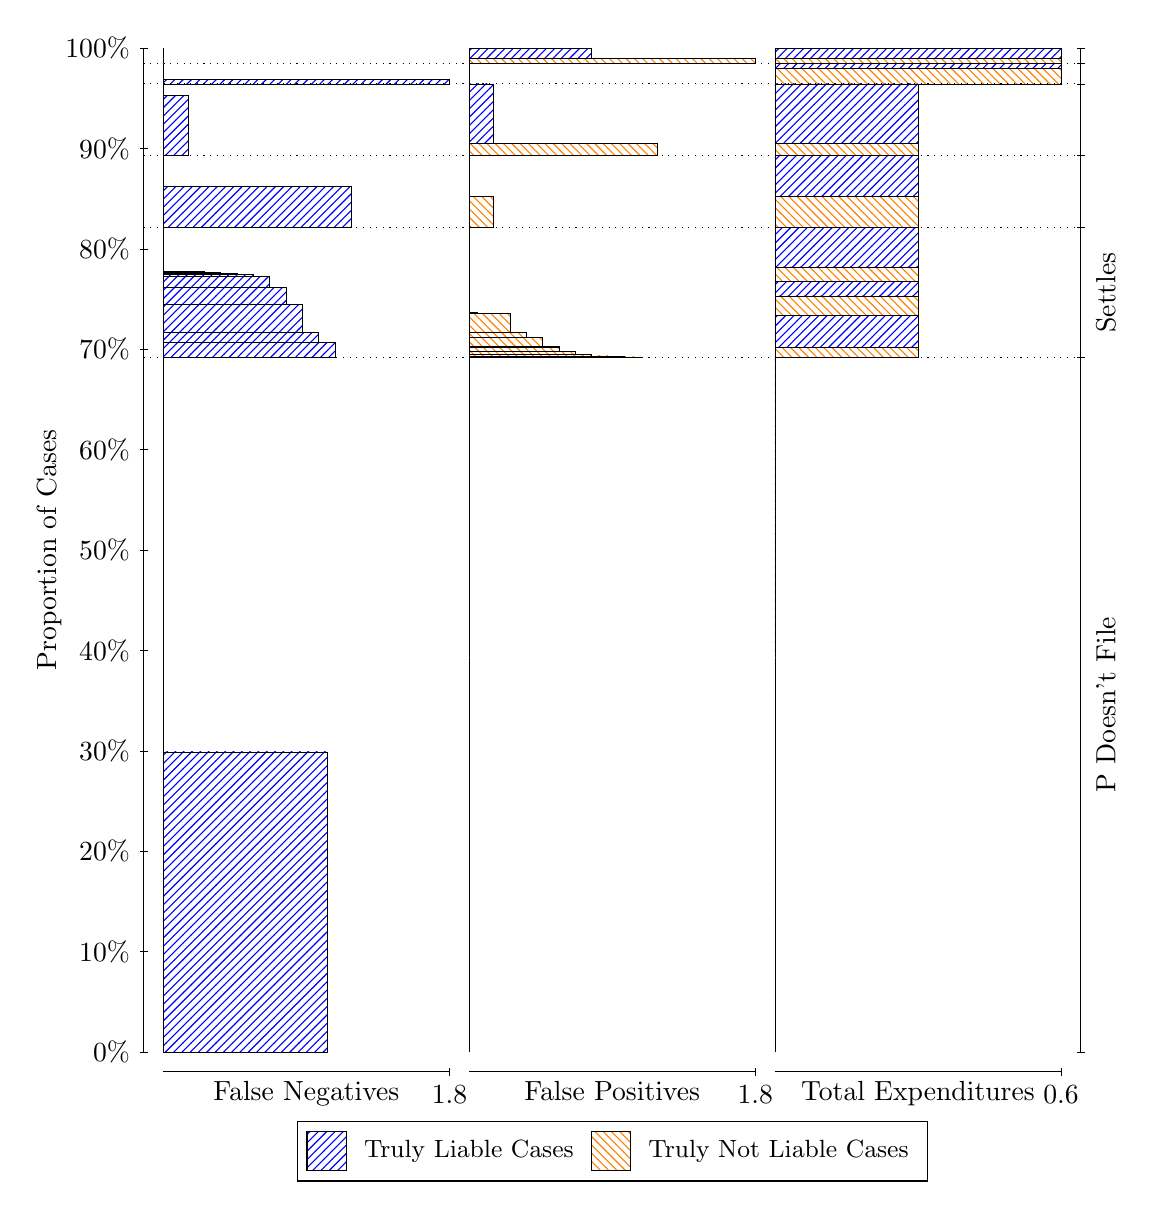
\begin{tikzpicture}
\draw[black, very thin] (1.5,1.75) -- (1.5,14.5);
\node[rotate=90, anchor=center] at (0.3, 8.125) {Proportion of Cases};
\draw[black, very thin] (1.45,1.75) -- (1.55,1.75);
\node[anchor=east] at (1.45, 1.75) {0\%};
\draw[black, very thin] (1.45,3.025) -- (1.55,3.025);
\node[anchor=east] at (1.45, 3.025) {10\%};
\draw[black, very thin] (1.45,4.3) -- (1.55,4.3);
\node[anchor=east] at (1.45, 4.3) {20\%};
\draw[black, very thin] (1.45,5.575) -- (1.55,5.575);
\node[anchor=east] at (1.45, 5.575) {30\%};
\draw[black, very thin] (1.45,6.85) -- (1.55,6.85);
\node[anchor=east] at (1.45, 6.85) {40\%};
\draw[black, very thin] (1.45,8.125) -- (1.55,8.125);
\node[anchor=east] at (1.45, 8.125) {50\%};
\draw[black, very thin] (1.45,9.4) -- (1.55,9.4);
\node[anchor=east] at (1.45, 9.4) {60\%};
\draw[black, very thin] (1.45,10.675) -- (1.55,10.675);
\node[anchor=east] at (1.45, 10.675) {70\%};
\draw[black, very thin] (1.45,11.95) -- (1.55,11.95);
\node[anchor=east] at (1.45, 11.95) {80\%};
\draw[black, very thin] (1.45,13.225) -- (1.55,13.225);
\node[anchor=east] at (1.45, 13.225) {90\%};
\draw[black, very thin] (1.45,14.5) -- (1.55,14.5);
\node[anchor=east] at (1.45, 14.5) {100\%};

\draw[black, very thin] (13.4,1.75) -- (13.4,14.5);
\draw[black, very thin] (13.35,1.75) -- (13.45,1.75);
\node[anchor=west] at (13.35, 1.75) {};
\draw[black, very thin] (13.35,10.573) -- (13.45,10.573);
\node[anchor=west] at (13.35, 10.573) {};
\draw[black, very thin] (13.35,12.22) -- (13.45,12.22);
\node[anchor=west] at (13.35, 12.22) {};
\draw[black, very thin] (13.35,13.138) -- (13.45,13.138);
\node[anchor=west] at (13.35, 13.138) {};
\draw[black, very thin] (13.35,14.045) -- (13.45,14.045);
\node[anchor=west] at (13.35, 14.045) {};
\draw[black, very thin] (13.35,14.304) -- (13.45,14.304);
\node[anchor=west] at (13.35, 14.304) {};
\draw[black, very thin] (13.35,14.5) -- (13.45,14.5);
\node[anchor=west] at (13.35, 14.5) {};

\draw[black, very thin, pattern color=blue, pattern=north east lines] (1.75,1.75) rectangle (3.8262,5.5606);
\draw[black, very thin, pattern color=orange, pattern=north west lines] (1.75,5.5606) rectangle (1.75,10.573);
\draw[black, very thin, pattern color=blue, pattern=north east lines] (1.75,10.573) rectangle (3.93,10.757);
\draw[black, very thin, pattern color=blue, pattern=north east lines] (1.75,10.757) rectangle (3.7224,10.893);
\draw[black, very thin, pattern color=blue, pattern=north east lines] (1.75,10.893) rectangle (3.5148,11.247);
\draw[black, very thin, pattern color=blue, pattern=north east lines] (1.75,11.247) rectangle (3.3071,11.463);
\draw[black, very thin, pattern color=blue, pattern=north east lines] (1.75,11.463) rectangle (3.0995,11.601);
\draw[black, very thin, pattern color=blue, pattern=north east lines] (1.75,11.601) rectangle (2.8919,11.625);
\draw[black, very thin, pattern color=blue, pattern=north east lines] (1.75,11.625) rectangle (2.6843,11.641);
\draw[black, very thin, pattern color=blue, pattern=north east lines] (1.75,11.641) rectangle (2.4767,11.649);
\draw[black, very thin, pattern color=blue, pattern=north east lines] (1.75,11.649) rectangle (2.269,11.659);
\draw[black, very thin, pattern color=orange, pattern=north west lines] (1.75,11.659) rectangle (1.75,12.22);
\draw[black, very thin, pattern color=blue, pattern=north east lines] (1.75,12.22) rectangle (4.1376,12.744);
\draw[black, very thin, pattern color=orange, pattern=north west lines] (1.75,12.744) rectangle (1.75,13.138);
\draw[black, very thin, pattern color=blue, pattern=north east lines] (1.75,13.138) rectangle (2.0614,13.896);
\draw[black, very thin, pattern color=orange, pattern=north west lines] (1.75,13.896) rectangle (1.75,14.045);
\draw[black, very thin, pattern color=blue, pattern=north east lines] (1.75,14.045) rectangle (5.3833,14.106);
\draw[black, very thin, pattern color=orange, pattern=north west lines] (1.75,14.106) rectangle (1.75,14.304);
\draw[black, very thin, pattern color=orange, pattern=north west lines] (1.75,14.304) rectangle (1.75,14.364);
\draw[black, very thin, pattern color=blue, pattern=north east lines] (1.75,14.364) rectangle (1.75,14.5);
\draw[black, very thin, pattern color=orange, pattern=north west lines] (5.6333,1.75) rectangle (5.6333,6.762);
\draw[black, very thin, pattern color=blue, pattern=north east lines] (5.6333,6.762) rectangle (5.6333,10.573);
\draw[black, very thin, pattern color=orange, pattern=north west lines] (5.6333,10.573) rectangle (7.8133,10.578);
\draw[black, very thin, pattern color=orange, pattern=north west lines] (5.6333,10.578) rectangle (7.6057,10.582);
\draw[black, very thin, pattern color=orange, pattern=north west lines] (5.6333,10.582) rectangle (7.3981,10.591);
\draw[black, very thin, pattern color=orange, pattern=north west lines] (5.6333,10.591) rectangle (7.1905,10.605);
\draw[black, very thin, pattern color=orange, pattern=north west lines] (5.6333,10.605) rectangle (6.9829,10.649);
\draw[black, very thin, pattern color=orange, pattern=north west lines] (5.6333,10.649) rectangle (6.7752,10.701);
\draw[black, very thin, pattern color=orange, pattern=north west lines] (5.6333,10.701) rectangle (6.7752,10.709);
\draw[black, very thin, pattern color=orange, pattern=north west lines] (5.6333,10.709) rectangle (6.5676,10.823);
\draw[black, very thin, pattern color=orange, pattern=north west lines] (5.6333,10.823) rectangle (6.36,10.886);
\draw[black, very thin, pattern color=orange, pattern=north west lines] (5.6333,10.886) rectangle (6.1524,11.133);
\draw[black, very thin, pattern color=blue, pattern=north east lines] (5.6333,11.133) rectangle (5.7371,11.143);
\draw[black, very thin, pattern color=blue, pattern=north east lines] (5.6333,11.143) rectangle (5.6333,12.22);
\draw[black, very thin, pattern color=orange, pattern=north west lines] (5.6333,12.22) rectangle (5.9448,12.614);
\draw[black, very thin, pattern color=blue, pattern=north east lines] (5.6333,12.614) rectangle (5.6333,13.138);
\draw[black, very thin, pattern color=orange, pattern=north west lines] (5.6333,13.138) rectangle (8.021,13.288);
\draw[black, very thin, pattern color=blue, pattern=north east lines] (5.6333,13.288) rectangle (5.9448,14.045);
\draw[black, very thin, pattern color=orange, pattern=north west lines] (5.6333,14.045) rectangle (5.6333,14.244);
\draw[black, very thin, pattern color=blue, pattern=north east lines] (5.6333,14.244) rectangle (5.6333,14.304);
\draw[black, very thin, pattern color=orange, pattern=north west lines] (5.6333,14.304) rectangle (9.2667,14.364);
\draw[black, very thin, pattern color=blue, pattern=north east lines] (5.6333,14.364) rectangle (7.1905,14.5);
\draw[black, very thin, pattern color=orange, pattern=north west lines] (9.5167,1.75) rectangle (9.5167,6.762);
\draw[black, very thin, pattern color=blue, pattern=north east lines] (9.5167,6.762) rectangle (9.5167,10.573);
\draw[black, very thin, pattern color=orange, pattern=north west lines] (9.5167,10.573) rectangle (11.333,10.701);
\draw[black, very thin, pattern color=blue, pattern=north east lines] (9.5167,10.701) rectangle (11.333,11.104);
\draw[black, very thin, pattern color=orange, pattern=north west lines] (9.5167,11.104) rectangle (11.333,11.352);
\draw[black, very thin, pattern color=blue, pattern=north east lines] (9.5167,11.352) rectangle (11.333,11.536);
\draw[black, very thin, pattern color=orange, pattern=north west lines] (9.5167,11.536) rectangle (11.333,11.721);
\draw[black, very thin, pattern color=blue, pattern=north east lines] (9.5167,11.721) rectangle (11.333,12.22);
\draw[black, very thin, pattern color=orange, pattern=north west lines] (9.5167,12.22) rectangle (11.333,12.614);
\draw[black, very thin, pattern color=blue, pattern=north east lines] (9.5167,12.614) rectangle (11.333,13.138);
\draw[black, very thin, pattern color=orange, pattern=north west lines] (9.5167,13.138) rectangle (11.333,13.288);
\draw[black, very thin, pattern color=blue, pattern=north east lines] (9.5167,13.288) rectangle (11.333,14.045);
\draw[black, very thin, pattern color=orange, pattern=north west lines] (9.5167,14.045) rectangle (13.15,14.244);
\draw[black, very thin, pattern color=blue, pattern=north east lines] (9.5167,14.244) rectangle (13.15,14.304);
\draw[black, very thin, pattern color=orange, pattern=north west lines] (9.5167,14.304) rectangle (13.15,14.364);
\draw[black, very thin, pattern color=blue, pattern=north east lines] (9.5167,14.364) rectangle (13.15,14.5);
\draw[black, dotted] (1.5,10.573) -- (13.4,10.573);
\draw[black, dotted] (1.5,12.22) -- (13.4,12.22);
\draw[black, dotted] (1.5,13.138) -- (13.4,13.138);
\draw[black, dotted] (1.5,14.045) -- (13.4,14.045);
\draw[black, dotted] (1.5,14.304) -- (13.4,14.304);
\draw[black, very thin] (1.75,1.5) -- (5.3833,1.5);
\node[anchor=north] at (3.5667, 1.5) {False Negatives};
\draw[black, very thin] (5.3833,1.45) -- (5.3833,1.55);
\node[anchor=north] at (5.3833, 1.45) {1.8};

\draw[black, very thin] (5.6333,1.5) -- (9.2667,1.5);
\node[anchor=north] at (7.45, 1.5) {False Positives};
\draw[black, very thin] (9.2667,1.45) -- (9.2667,1.55);
\node[anchor=north] at (9.2667, 1.45) {1.8};

\draw[black, very thin] (9.5167,1.5) -- (13.15,1.5);
\node[anchor=north] at (11.333, 1.5) {Total Expenditures};
\draw[black, very thin] (13.15,1.45) -- (13.15,1.55);
\node[anchor=north] at (13.15, 1.45) {0.6};

\node[black, centered, rotate=90] at (13.72, 6.1613) {P Doesn't File};
\node[black, centered, rotate=90] at (13.72, 11.396) {Settles};





\draw (7.449999999999999,1.5) node[draw=none] (baseCoordinate) {};
\begin{scope}[align=center]
        \matrix[scale=0.5, draw=black, below=0.5cm of baseCoordinate, nodes={draw}, column sep=0.1cm]{
            \node[rectangle, draw, minimum width=0.5cm, minimum height=0.5cm, pattern=north east lines, pattern color=blue] {}; &
            \node[draw=none, font=\small] (B) {Truly Liable Cases}; &
            \node[rectangle, draw, minimum width=0.5cm, minimum height=0.5cm, pattern=north west lines, pattern color=orange] {}; &
            \node[draw=none, font=\small] (B) {Truly Not Liable Cases}; \\
            };
\end{scope}

\end{tikzpicture}
\end{document}